\documentclass[11pt]{article}

\emergencystretch=2em

\usepackage[margin=0.75in]{geometry}
\usepackage{amsmath, amssymb}
\usepackage{graphicx}
\usepackage{caption}
\usepackage{booktabs}
\usepackage{hyperref}
\hypersetup{hypertexnames=false}
\usepackage{cleveref}
\usepackage{siunitx}
\usepackage{bm}
\usepackage{algorithm}
\usepackage{algpseudocode}
\usepackage[numbers,sort&compress]{natbib}

\graphicspath{{outputs/paper_figures/}}

\title{Dower Coppler: A Multi-Lag Coherence-Weighted Signed Doppler Index}

\author{}

\date{}

\begin{document}

\twocolumn[{%
\maketitle

\begin{center}
  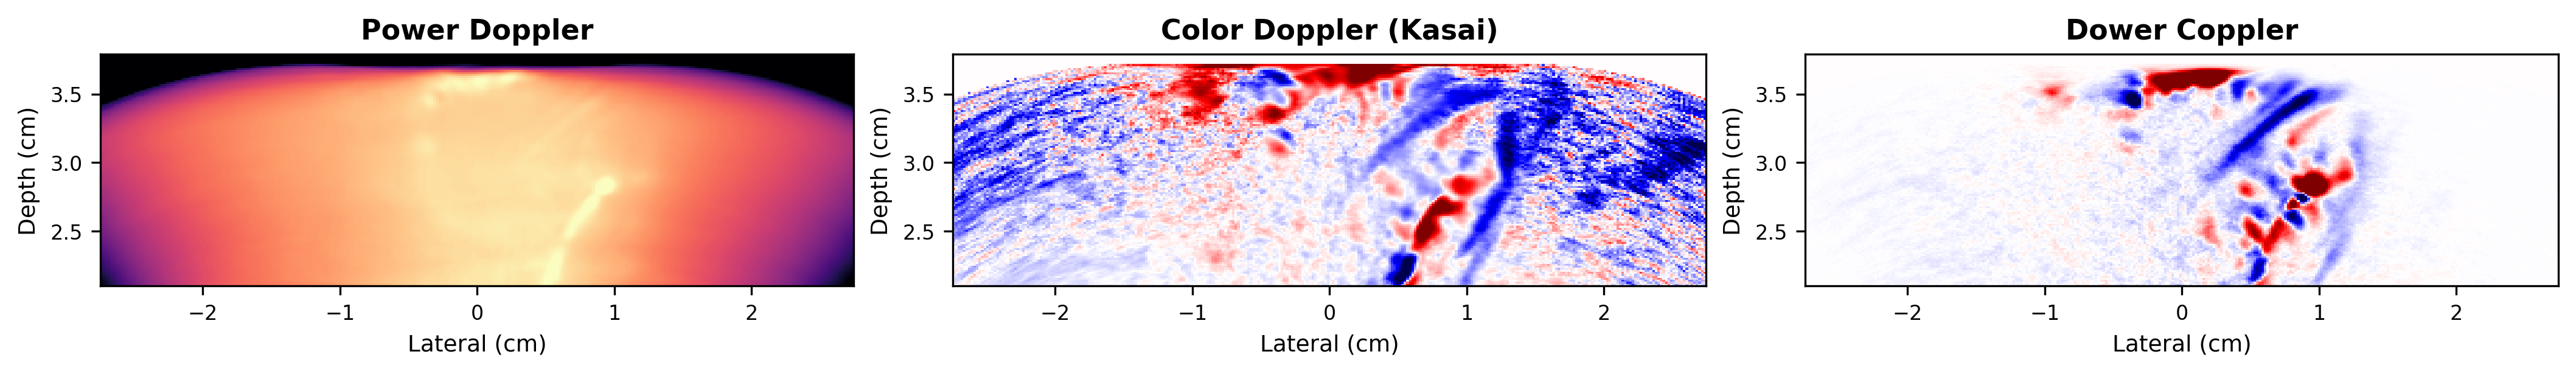
\includegraphics[width=\textwidth]{fig_three_panel_comparison.png}
\end{center}
\vspace{0.5em}

\begin{abstract}
Ultrafast power Doppler imaging is sensitive to weak flow but discards
flow direction, while classic autocorrelation color Doppler estimates
signed velocity from phase and is sensitive to noise.  We propose
\textbf{Dower Coppler}, a composite signed Doppler index for
SVD-filtered ultrafast compound data.  The method does not introduce a
new Doppler estimator from first principles; instead, it combines known
building blocks---complex autocorrelation, multi-lag phase regression,
power-like magnitude weighting, and fit-quality gating---into a single
scalar image.  For each pixel, we estimate the beam-projected phase
velocity $v_\phi$ from a weighted multi-lag phase fit, then multiply it
by the geometric mean of the lag-correlation magnitudes and by the
weighted $R^2$ of the phase fit, yielding
$v_\phi\,\mathrm{gmean}_k(|R_k|)\,R^2$.  In
Monte~Carlo simulations across five noise and interference scenarios,
the multi-lag phase estimator reduces median absolute frequency error
by 2--3$\times$ relative to the Kasai estimator.  We demonstrate the method
\textit{in~vivo} on transcranial functional ultrasound data acquired
from human cortex through the intact skull, without a cranial window,
where the Dower Coppler index reveals opposing flow directions in
adjacent vessels that are invisible in conventional power Doppler.
\end{abstract}

\vspace{0.5em}
}]

% ========================================================================
\section{Introduction}
\label{sec:intro}
% ========================================================================

Ultrafast ultrasound imaging, in which the entire field of view is
insonified by unfocused or plane-wave transmissions at kilohertz frame
rates, has enabled a new class of hemodynamic imaging
modalities~\cite{demene2015svd,tremblaydarveau2017coherencepd}.  Transcranial
functional ultrasound (fUS) exploits this capability to image cerebral
blood flow through the intact skull, but the transcranial setting
imposes severe SNR constraints due to skull attenuation and
aberration.  Spatiotemporal SVD clutter filtering is now a standard
preprocessing step in ultrafast Doppler and fUS because it separates
tissue and blood components using their different spatiotemporal
coherence~\cite{demene2015svd}.  After clutter filtering, the most
common flow-strength image is power Doppler, which displays integrated
Doppler power rather than mean Doppler frequency~\cite{rubin1994powerdoppler}.
Power Doppler is robust and straightforward to compute, but it discards
phase information: the resulting image is unsigned and carries no
information about flow velocity or direction.

The Kasai autocorrelator~\cite{kasai1985autocorrelation} recovers a
signed velocity estimate from the phase of the lag-1 autocorrelation,
$\angle R_1$, and complex autocorrelation methods form the classical
foundation of color flow imaging.  Extensions using arbitrary spatial
and temporal autocorrelation lags have also been studied in the color
flow literature~\cite{torp1994autocorrelation}.  Thus, neither SVD
clutter filtering, autocorrelation velocity estimation, nor the use of
multiple lags is new by itself.  The practical problem we address is how
to combine signed phase information with a power-like confidence image
for low-SNR transcranial ultrafast data.

Shen and Guo~\cite{shen2022tmas} introduced temporal
multiply-and-sum (TMAS), the direct product-of-lag-magnitudes precursor
to our coherence term, showing that multiplicative combinations of
slow-time autocorrelations can improve power Doppler signal-to-noise
ratio.
Motivated by that idea, we use multi-lag autocorrelations to separate
coherent flow from incoherent background.  Rather than multiplying all
lag magnitudes directly, we use their geometric mean as a bounded
coherence term.  This keeps the lag-product intuition---pixels must be
temporally coherent across multiple lags---without the rapidly growing
dynamic range of a raw product.  On its own, however, any
magnitude-only lag statistic inherits the fundamental limitation of
power Doppler: it discards phase and produces an unsigned map.

A natural remedy is to use the autocorrelation phases, not just the
magnitudes.  For a coherent scatterer moving at angular frequency
$\omega$, the lag-$k$ autocorrelation satisfies $\angle R_k \approx
\omega k$: the phase is linear in lag.  Fitting a line to
$\{\angle R_k\}_{k=1}^{K}$ yields a multi-lag frequency estimate that
uses all available lags rather than just lag~1.  The idea of
estimating frequency from the slope of autocorrelation phase is
classical---Tretter~\cite{tretter1985phaseregression} analyzed its
statistical properties, and Fitz~\cite{fitz1994frequency} developed
fast approximations.  Dower Coppler should therefore be viewed as a
composite Doppler index, not a new physical Doppler estimator from first
principles.

In this paper we propose \textbf{Dower Coppler}: a multi-lag,
coherence-weighted signed Doppler index.  It uses the signed axial
phase velocity from a weighted multi-lag phase regression, multiplied by
two confidence factors: the geometric mean of the lag-correlation
magnitudes and the weighted $R^2$ of the phase-versus-lag fit.  The
regression weights are the autocorrelation magnitudes~$|R_k|$, so that
lags with stronger signal dominate the fitted phase slope, while pixels
whose phase is not approximately linear in lag are attenuated by the
fit-quality term.  The distinctive contribution is this specific
scalar product, $v_\phi\,G_R\,R^2$, for SVD-filtered ultrafast compound
data.

The experimental setting is also relevant.  Prior human fUS studies
have primarily used intraoperative imaging after skull opening
\cite{imbault2017intraoperative} or imaging through acoustically
transparent cranial implants/windows
\cite{rabut2024cranialwindow,soloukey2025mobile}.  Here, the data are
acquired transcranially through the intact adult skull.  This extreme
low-SNR operating point motivates a conservative composite index that
uses multi-lag evidence and explicit phase-fit quality rather than a
single-lag color Doppler estimate alone.

We evaluate the index and its phase-velocity component in two settings: (1)~Monte Carlo simulations
under additive white Gaussian noise, decorrelation, lag outliers,
clutter leakage, and mixed-flow scenarios; and (2)~\textit{in~vivo}
transcranial functional ultrasound imaging of human cortex.
\Cref{fig:invivo_comparison} previews the key result.


% ========================================================================
\section{Methods}
\label{sec:methods}
% ========================================================================

\subsection{Signal Model}
\label{sec:signal_model}

Let $s_t(\bm{x})$ denote the clutter-filtered complex analytic signal
at pixel~$\bm{x}$ and slow-time frame~$t$, where $t = 0, 1, \ldots,
T{-}1$.  For a coherent scatterer population moving at a constant
Doppler angular frequency~$\omega$, the idealized signal is
\begin{equation}
  s_t = A \, e^{j(\omega t + \phi_0)} + n_t,
  \label{eq:signal_model}
\end{equation}
where $A$ is the (real, positive) amplitude, $\phi_0$ is an arbitrary
initial phase, and $n_t$ is zero-mean additive noise.

The lag-$k$ temporal autocorrelation is
\begin{equation}
  R_k(\bm{x})
  = \frac{1}{T - k} \sum_{t=0}^{T-k-1}
    s_{t+k}(\bm{x})\, s_t^*(\bm{x}).
  \label{eq:autocorr}
\end{equation}
In the noiseless, fully coherent case,
$R_k \approx |A|^2 e^{j \omega k}$, so that
\begin{equation}
  \angle R_k \approx \omega k.
  \label{eq:phase_linear}
\end{equation}

\subsection{Background: Multi-Lag Coherence}
\label{sec:tmas_background}

Standard power Doppler uses the zero-lag power $|R_0| =
\frac{1}{T}\sum_t |s_t|^2$.  A TMAS-style product of
autocorrelation magnitudes across lags $k = 1, \ldots, K$ is
\begin{equation}
  M_{\text{TMAS}} = \prod_{k=1}^{K} |R_k|.
  \label{eq:tmas}
\end{equation}
This construction is motivated by the TMAS product of autocorrelation
magnitudes~\cite{shen2022tmas}.
Because $|R_k|$ decays with lag for uncorrelated noise but remains
roughly constant for coherent flow, the product suppresses background
more strongly than $|R_0|$ alone.  In the current Dower Coppler
implementation, we use the geometric mean of the same lag magnitudes,
\begin{equation}
  G_R =
  \exp\!\left(\frac{1}{K}\sum_{k=1}^{K}\log\left(\max(|R_k|,\epsilon)\right)\right),
  \label{eq:geomean_r}
\end{equation}
with $\epsilon=10^{-30}$ for numerical stability.  This preserves the
multi-lag coherence weighting while keeping the scale comparable to a
single autocorrelation magnitude.  Like the raw TMAS product, $G_R$ is
non-negative and therefore carries no directional information.

\subsection{Multi-Lag Phase Regression}
\label{sec:phase_regression}

We estimate the Doppler frequency from the slope of autocorrelation
phase versus lag.  Given the unwrapped phases
\begin{equation}
  \phi_k = \operatorname{unwrap}\bigl(\angle R_k\bigr),
  \quad k = 1, \ldots, K,
\end{equation}
we seek the angular frequency~$\hat\omega$ that minimizes a weighted
residual.  The regression is constrained through the origin ($\phi_0 =
0$ at lag~$0$), since $R_0$ is real and positive after clutter
filtering.

\paragraph{Plain weighted least squares (WLS).}
The initial estimate uses the autocorrelation magnitudes as weights:
\begin{equation}
  \hat\omega_{\text{WLS}}
  = \frac{\sum_{k=1}^K |R_k|\, k\, \phi_k}
         {\sum_{k=1}^K |R_k|\, k^2}.
  \label{eq:wls}
\end{equation}
This is the weighted regression of~$\phi_k$ on~$k$ through the
origin, where lags with stronger autocorrelation contribute more.

\paragraph{Fit quality.}
We quantify whether the phase sequence is well described by a single
linear slope using a weighted coefficient of determination.  With
\begin{equation}
  \bar{\phi} = \frac{\sum_k |R_k|\,\phi_k}{\sum_k |R_k|},
\end{equation}
we compute
\begin{align}
  \mathrm{SSE} &= \sum_k |R_k|\,(\phi_k-\hat\omega_{\mathrm{WLS}} k)^2,\\
  \mathrm{SST} &= \sum_k |R_k|\,(\phi_k-\bar{\phi})^2,
\end{align}
and
\begin{equation}
  Q = R^2 =
  \operatorname{clamp}\!\left(1-\frac{\mathrm{SSE}}{\max(\mathrm{SST},10^{-12})},0,1\right).
  \label{eq:phase_r2}
\end{equation}
Pixels with weak lag correlations or inconsistent phase evolution
therefore receive low weight in the final image.

\subsection{Dower Coppler}
\label{sec:signed_tmas}

The Dower Coppler index combines the signed velocity estimated from the
multi-lag phase slope with the multi-lag coherence and fit-quality
terms.  First, the phase slope in radians per slow-time frame is
converted to a beam-projected axial phase velocity:
\begin{equation}
  v_\phi =
  \hat\omega_{\mathrm{WLS}}\,
  \frac{f_{\mathrm{slow}}}{2\pi}\,
  \frac{c}{2 f_0},
  \label{eq:phase_velocity}
\end{equation}
where $f_{\mathrm{slow}}$ is the cadence of the slow-time samples, $c$
is the assumed speed of sound, and $f_0$ is the transmit center
frequency.  For compounded plane-wave data, $f_{\mathrm{slow}}$ is the
transmit pulse repetition frequency divided by the number of
transmissions per compounded frame.  This is the standard axial
Doppler conversion; no beam-flow angle correction is applied.  The final image is
\begin{equation}
  I_{\text{Dower}} = v_\phi \; G_R \; Q.
  \label{eq:dower}
\end{equation}
The result is positive for one axial flow direction and negative for
the opposite direction, depending on the system sign convention.  The
sign comes from $v_\phi$, while $G_R$ and $Q$ attenuate pixels with
weak temporal coherence or poor phase linearity.  Because $G_R$ is
signal-scale dependent, $I_{\text{Dower}}$ should be interpreted as a
signed Doppler evidence index rather than a quantitative velocity map;
$v_\phi$ is retained separately when velocity is the quantity of
interest.

The per-pixel computational cost is small: the autocorrelations
$R_k$ are computed for $K$~lags, followed by closed-form weighted
least squares and a weighted $R^2$ calculation.

\subsection{Phase Unwrapping}
\label{sec:unwrapping}

The autocorrelation phases $\angle R_k$ are individually wrapped to
$(-\pi, \pi]$.  Before regression, we apply a one-dimensional temporal
unwrap along the lag axis: for each consecutive pair of lags, the
phase difference is corrected to lie within $(-\pi, \pi]$ by adding
integer multiples of~$2\pi$.  This is a standard 1-D unwrap and does
not require spatial information.

The final $R^2$ quality term attenuates isolated unwrapping failures:
a miswrapped lag produces a large residual from the linear phase model,
lowering the weighted fit quality for that pixel.


% ========================================================================
\section{Simulation Study}
\label{sec:simulations}
% ========================================================================

\subsection{Setup}

We evaluate the phase slope estimators on synthetic slow-time
ensembles of $T = 64$ frames.  For each trial, a coherent signal is
generated according to \cref{eq:signal_model} with unit amplitude and
additive complex Gaussian noise at a specified SNR.  The true angular
frequency~$\omega$ is drawn from the set $\{0.35, 0.8, 1.35\}$~rad/frame,
and the SNR ranges from $-12$ to $+12$~dB.  We compute lag
autocorrelations up to $K = 5$ and run $N = 1024$ independent trials
per condition.

Five scenarios are tested:
\begin{enumerate}
  \item \textbf{AWGN}: coherent flow plus white Gaussian noise.
  \item \textbf{Decorrelation}: flow with a slow phase random walk
    (models scatterer turnover).
  \item \textbf{Lag outlier}: one high-lag autocorrelation is
    corrupted by a large additive phase error.
  \item \textbf{Clutter leakage}: a residual slow-moving clutter
    component is added to the flow signal.
  \item \textbf{Two-component flow}: a weaker flow component with the
    opposite sign is mixed with the primary flow.
\end{enumerate}

\subsection{Estimators Compared}

\begin{itemize}
  \item \textbf{Kasai}: $\hat\omega = \angle R_1$ (single-lag baseline).
  \item \textbf{WLS}: weighted least-squares phase slope
    (\cref{eq:wls}).
  \item \textbf{Huber-WLS}: robust comparison estimator using Huber
    residual weights ($\delta = 0.7$, 5~iterations).
  \item \textbf{Circular-sign-WLS}: direction from a circular
    objective $\arg\max_\omega \sum_k |R_k| \cos(\phi_k - \omega k)$,
    magnitude from WLS.
\end{itemize}

\subsection{Metrics}

For each estimator, we report:
\begin{itemize}
  \item \textbf{Median absolute error} (rad): median of $|\hat\omega
    - \omega|$.
  \item \textbf{RMSE} (rad): root mean squared error of the frequency
    estimate.
  \item \textbf{Sign error rate}: fraction of trials where
    $\text{sgn}(\hat\omega) \neq \text{sgn}(\omega)$.
\end{itemize}


% ========================================================================
\section{In Vivo Experiment}
\label{sec:invivo}
% ========================================================================

\subsection{Ethics Approval}

Human imaging was performed under WCG IRB Protocol \#20254791.  The
volunteer provided informed consent prior to data acquisition.
Ultrasound acquisition was performed within the approved IRB safety
limits.

\subsection{Data Acquisition}

Transcranial functional ultrasound data were acquired from the
temporal lobe of one healthy volunteer using a Butterfly iQ+
point-of-care ultrasound probe operated with custom firmware.  The
probe was placed over the temporal acoustic window and the acquisition
was performed through the intact skull, without craniotomy,
cranioplasty, or another acoustic cranial window.  The source ultratrace
contained 480 acquisitions.  Each acquisition contained 700 compounded
slow-time frames formed from five azimuthal plane-wave transmissions
spanning $\pm 6^\circ$; two additional noise loops were stored in the
raw IQ data but were not used for Doppler processing.  The transmit
center frequency was \SI{2.75}{\mega\hertz} with three transmit cycles,
and the receive data were sampled at \SI{4.17}{\mega\hertz} after
decimation.  The HDF5 metadata report an empirical pulse-repetition
rate of \SI{1245.9}{\hertz} over the acquisition subset used for the
main figures; because each compounded frame used five transmit angles,
the corresponding compounded-frame cadence was approximately
\SI{249}{\hertz}.  The assumed sound speed was
\SI{1600}{\meter\per\second}.

The original beamformed volume covered
\SIrange{-27.456}{27.456}{\milli\meter} laterally,
\SIrange{-20}{20}{\milli\meter} elevationally, and
\SIrange{21.0}{37.896}{\milli\meter} in depth on a
$147 \times 30 \times 58$ lateral-elevation-depth grid.  The main
paper figures were generated from a fine lateral/depth rebeamform of
the two central elevation planes (original elevation indices 14 and
15), using acquisitions 200--399.  This figure dataset used a
$294 \times 2 \times 116$ lateral-elevation-depth grid over the same
lateral and depth extent.  The temporal-stability analysis used
precomputed per-buffer Doppler arrays and explicitly varied the number
of buffers included in the median.

\begin{table*}[t]
\centering
\caption{Key acquisition and reconstruction parameters for the
  transcranial human fUS dataset.}
\label{tab:invivo_params}
\small
\begin{tabular}{@{}ll@{}}
\toprule
Parameter & Value \\
\midrule
Target / window & Temporal lobe / temporal acoustic window \\
Probe & Butterfly iQ+ with custom firmware \\
Acquisitions in ultratrace & 480 \\
Frames per acquisition & 700 compounded slow-time frames \\
Transmit angles & 5 azimuthal angles over $\pm 6^\circ$ \\
Transmit frequency & \SI{2.75}{\mega\hertz}, 3 cycles \\
Empirical pulse PRF & \SI{1245.9}{\hertz} (acq. 200--399 mean) \\
Compounded-frame cadence & \SI{249}{\hertz} \\
Sampling rate & \SI{4.17}{\mega\hertz} after decimation \\
Depth range & \SIrange{21.0}{37.896}{\milli\meter} \\
Sound speed & \SI{1600}{\meter\per\second} \\
Original grid & $147 \times 30 \times 58$ (lat. $\times$ elev. $\times$ depth) \\
Figure grid & $294 \times 2 \times 116$ (lat. $\times$ elev. $\times$ depth) \\
\bottomrule
\end{tabular}
\end{table*}

\subsection{Processing Pipeline}

Clutter filtering was performed by singular value decomposition (SVD)
of the slow-time ensemble at each pixel, with low-rank tissue clutter
components removed.  In the current processing, the compound data are
mean-subtracted before SVD filtering; the lowest 8\% of singular modes
are removed, the high cutoff is 1.0, the fast SVD implementation is
used, and the first five filtered frames are omitted from Doppler
summaries and phase fitting.  Beamforming used the MACH GPU
delay-and-sum backend, channel mean subtraction, an $f$-number of 0.5,
all enabled receive rows, and one-row compounding.  The source
ultratrace was beamformed into 30 elevation planes with 20 processing
chunks; the fine-grid figure dataset used the two central elevation
planes at doubled lateral/depth sampling.  All Doppler estimators share
the same filtered ensemble; they differ only in how the filtered
slow-time data are reduced to an image.  We computed:
\begin{itemize}
  \item Standard power Doppler ($|R_0|$).
  \item Kasai color Doppler ($\angle R_1$).
  \item Multi-lag phase velocity from weighted phase regression.
  \item Dower Coppler, $v_\phi\,G_R\,R^2$, at $K = 5$.
\end{itemize}


% ========================================================================
\section{Results}
\label{sec:results}
% ========================================================================

\subsection{Simulation Results}

\Cref{tab:sim_results} summarizes the estimator performance across
all five scenarios.

\begin{table*}[t]
\centering
\caption{Estimator performance averaged over SNR and velocity
  conditions.  Best values in each scenario are shown in
  \textbf{bold}.}
\label{tab:sim_results}
\small
\begin{tabular}{@{}llccc@{}}
\toprule
Scenario & Estimator & Med.\ abs.\ err. & RMSE & Sign err. \\
         &           & (rad)             & (rad) & (\%) \\
\midrule
AWGN
  & Kasai      & 0.235 & 0.401 & 8.2 \\
  & WLS        & \textbf{0.095} & 0.257 & 6.8 \\
  & Huber-WLS  & 0.096 & 0.259 & 6.8 \\
  & Circ-WLS   & 0.101 & \textbf{0.253} & \textbf{6.5} \\
\midrule
Decorrelation
  & Kasai      & 0.243 & 0.415 & 8.4 \\
  & WLS        & \textbf{0.112} & 0.277 & 7.1 \\
  & Huber-WLS  & \textbf{0.112} & 0.278 & 7.0 \\
  & Circ-WLS   & 0.125 & \textbf{0.274} & \textbf{6.8} \\
\midrule
Lag outlier
  & Kasai      & 0.241 & 0.401 & 8.6 \\
  & WLS        & 0.094 & 0.276 & 6.5 \\
  & Huber-WLS  & \textbf{0.092} & \textbf{0.267} & 6.6 \\
  & Circ-WLS   & 0.105 & 0.271 & \textbf{6.4} \\
\midrule
Clutter leak
  & Kasai      & 0.380 & 0.546 & 10.0 \\
  & WLS        & 0.182 & 0.373 & 9.8 \\
  & Huber-WLS  & 0.180 & 0.374 & 9.6 \\
  & Circ-WLS   & \textbf{0.178} & \textbf{0.368} & \textbf{8.5} \\
\midrule
Two-component
  & Kasai      & 0.338 & 0.518 & 10.7 \\
  & WLS        & \textbf{0.128} & 0.315 & 9.0 \\
  & Huber-WLS  & \textbf{0.128} & 0.316 & 8.9 \\
  & Circ-WLS   & 0.133 & \textbf{0.308} & \textbf{8.3} \\
\bottomrule
\end{tabular}
\end{table*}

Across all scenarios, WLS and Huber-WLS reduce the median absolute
frequency error by approximately 2--3$\times$ relative to the Kasai
estimator.  In the clean AWGN case, WLS and Huber-WLS are nearly
identical, confirming that the robust reweighting does not degrade
performance when no outliers are present.  Under the lag-outlier
scenario, Huber-WLS achieves the lowest median error and RMSE, as the
Huber weights suppress the corrupted lag.  The circular-sign-WLS
hybrid consistently achieves the lowest sign error rate, particularly
under clutter leakage and two-component flow.

\subsection{In Vivo Results}

\begin{figure*}[t]
  \centering
  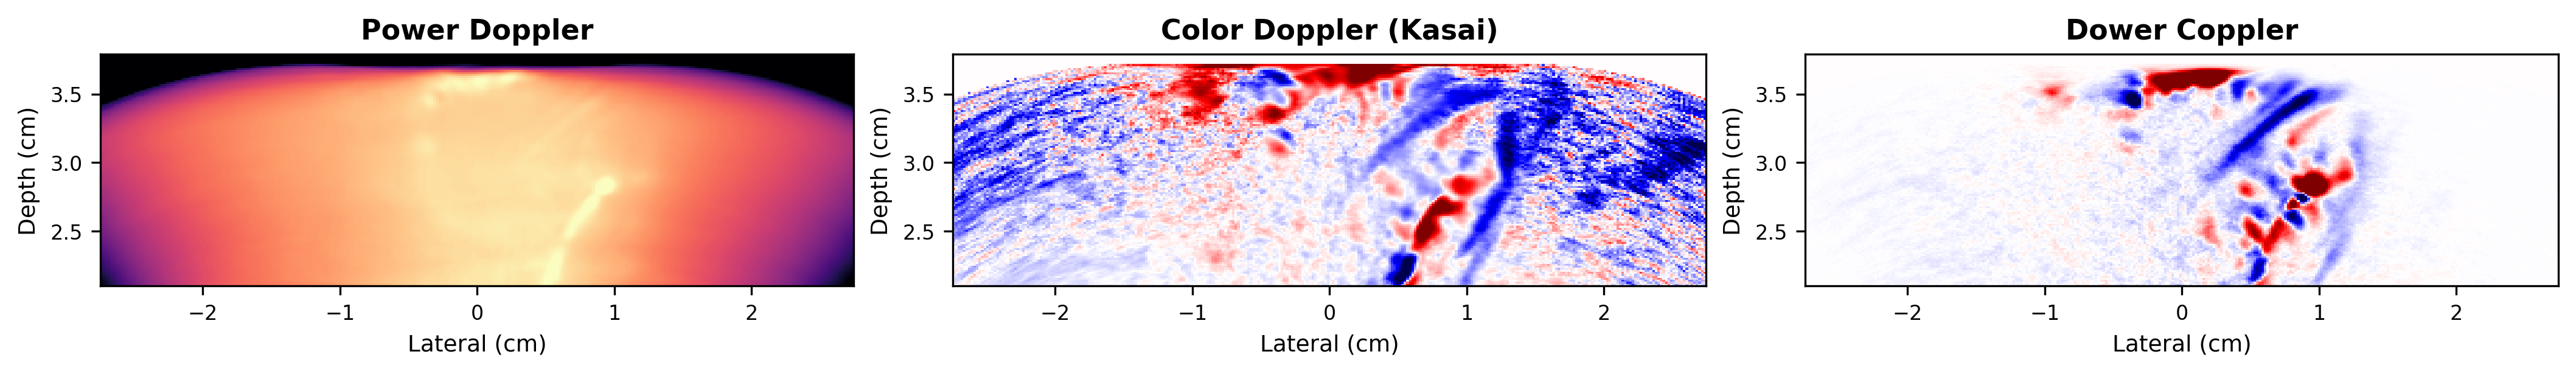
\includegraphics[width=\textwidth]{fig_three_panel_comparison.png}
  \caption{Transcranial cortex imaging (median of 480 Doppler buffers,
    plane-wave compounding).  \textbf{Left}: power Doppler, displayed
    from $-100$ to $140$~dB, shows vessel structure but no directional
    information.  \textbf{Center}: Kasai color Doppler ($\angle R_1$)
    reveals direction but is dominated by noise.  \textbf{Right}:
    Dower Coppler ($v_\phi\,G_R\,R^2$, $K=5$) combines multi-lag
    coherence weighting with directional information from the phase
    slope and fit quality.
    Opposing flow directions in adjacent cortical vessels are clearly
    resolved.}
  \label{fig:invivo_comparison}
\end{figure*}

As shown in \cref{fig:invivo_comparison}, power Doppler delineates the
cortical vasculature with high sensitivity but provides no directional
information.  Kasai color Doppler (center) reveals flow direction but
is dominated by noise, with vessel structure largely obscured.
The proposed Dower Coppler (right) attenuates incoherent pixels using
the multi-lag magnitude and fit-quality terms while recovering flow
direction from the multi-lag phase slope.  Adjacent cortical vessels with opposing flow
directions---invisible in power Doppler---are clearly separated in the
Dower Coppler image.

\Cref{fig:dower_ablation} isolates the contribution of the main
terms in the composite index.  The phase velocity $v_\phi$ alone
contains the directional pattern but also substantial background
phase noise.  Multiplication by the multi-lag coherence strength
$G_R$ suppresses decorrelated background and emphasizes vessel-like
structures.  Multiplication by $R^2$ preserves the signed velocity
interpretation while down-weighting pixels whose lag phases are poorly
explained by a single slope.  The $G_R$ panel shows that the magnitude
term is power-Doppler-like and unsigned; direction enters through
$v_\phi$.

\begin{figure*}[t]
  \centering
  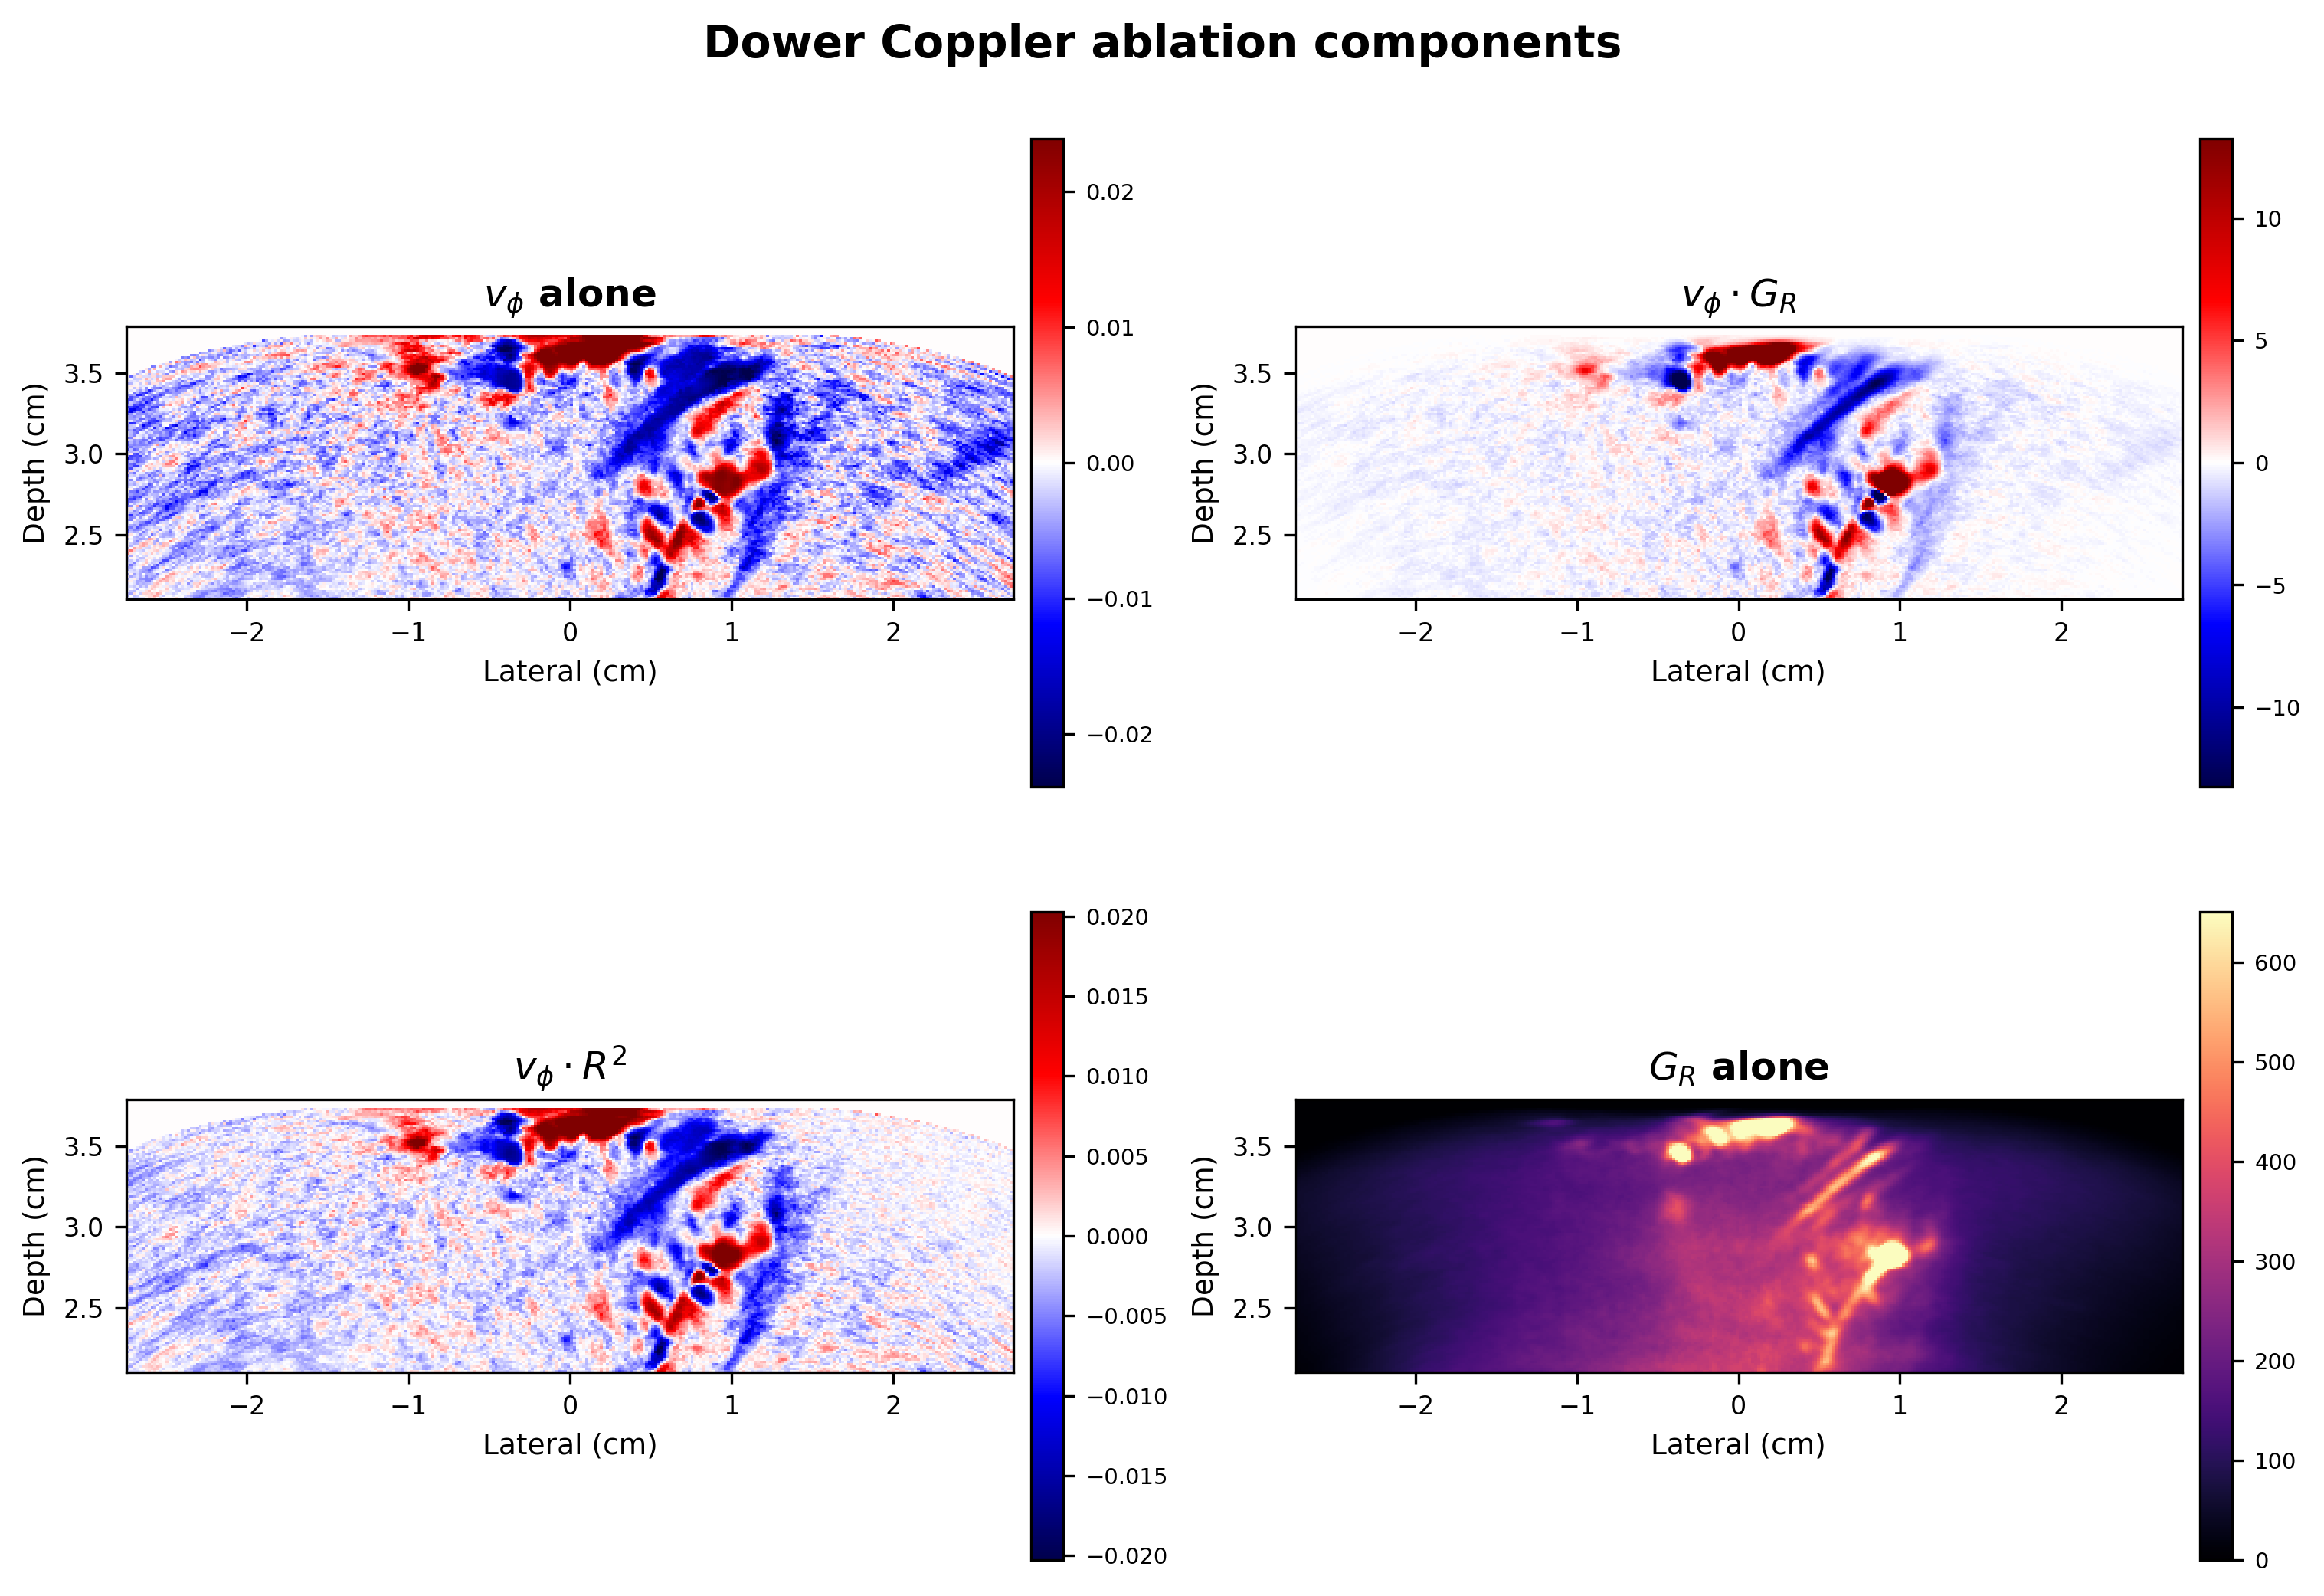
\includegraphics[width=\textwidth]{fig_dower_ablation.png}
  \caption{Ablation of the Dower Coppler components on the same
    transcranial image plane.  $v_\phi$ alone is the signed multi-lag
    phase-velocity estimate.  $v_\phi G_R$ adds the geometric mean of
    multi-lag autocorrelation magnitudes, suppressing incoherent
    background.  $v_\phi R^2$ gates the signed velocity by the
    phase-linearity fit quality.  $G_R$ alone is the unsigned
    coherence-strength image.  The final Dower Coppler image uses
    $v_\phi G_R R^2$.}
  \label{fig:dower_ablation}
\end{figure*}

\Cref{fig:velocity_vs_color} separates the signed velocity estimate
from the Dower Coppler amplitude weighting.  The multi-lag phase
velocity preserves the dominant flow-direction pattern seen by the
lag-1 Kasai estimator, but the Bland--Altman comparison shows that the
two velocity estimates are not interchangeable at high-magnitude
pixels.  In this dataset the mean bias is near zero, while the limits
of agreement are set by pixels where the lag-1 phase and the multi-lag
phase-slope fit disagree.

\begin{figure*}[t]
  \centering
  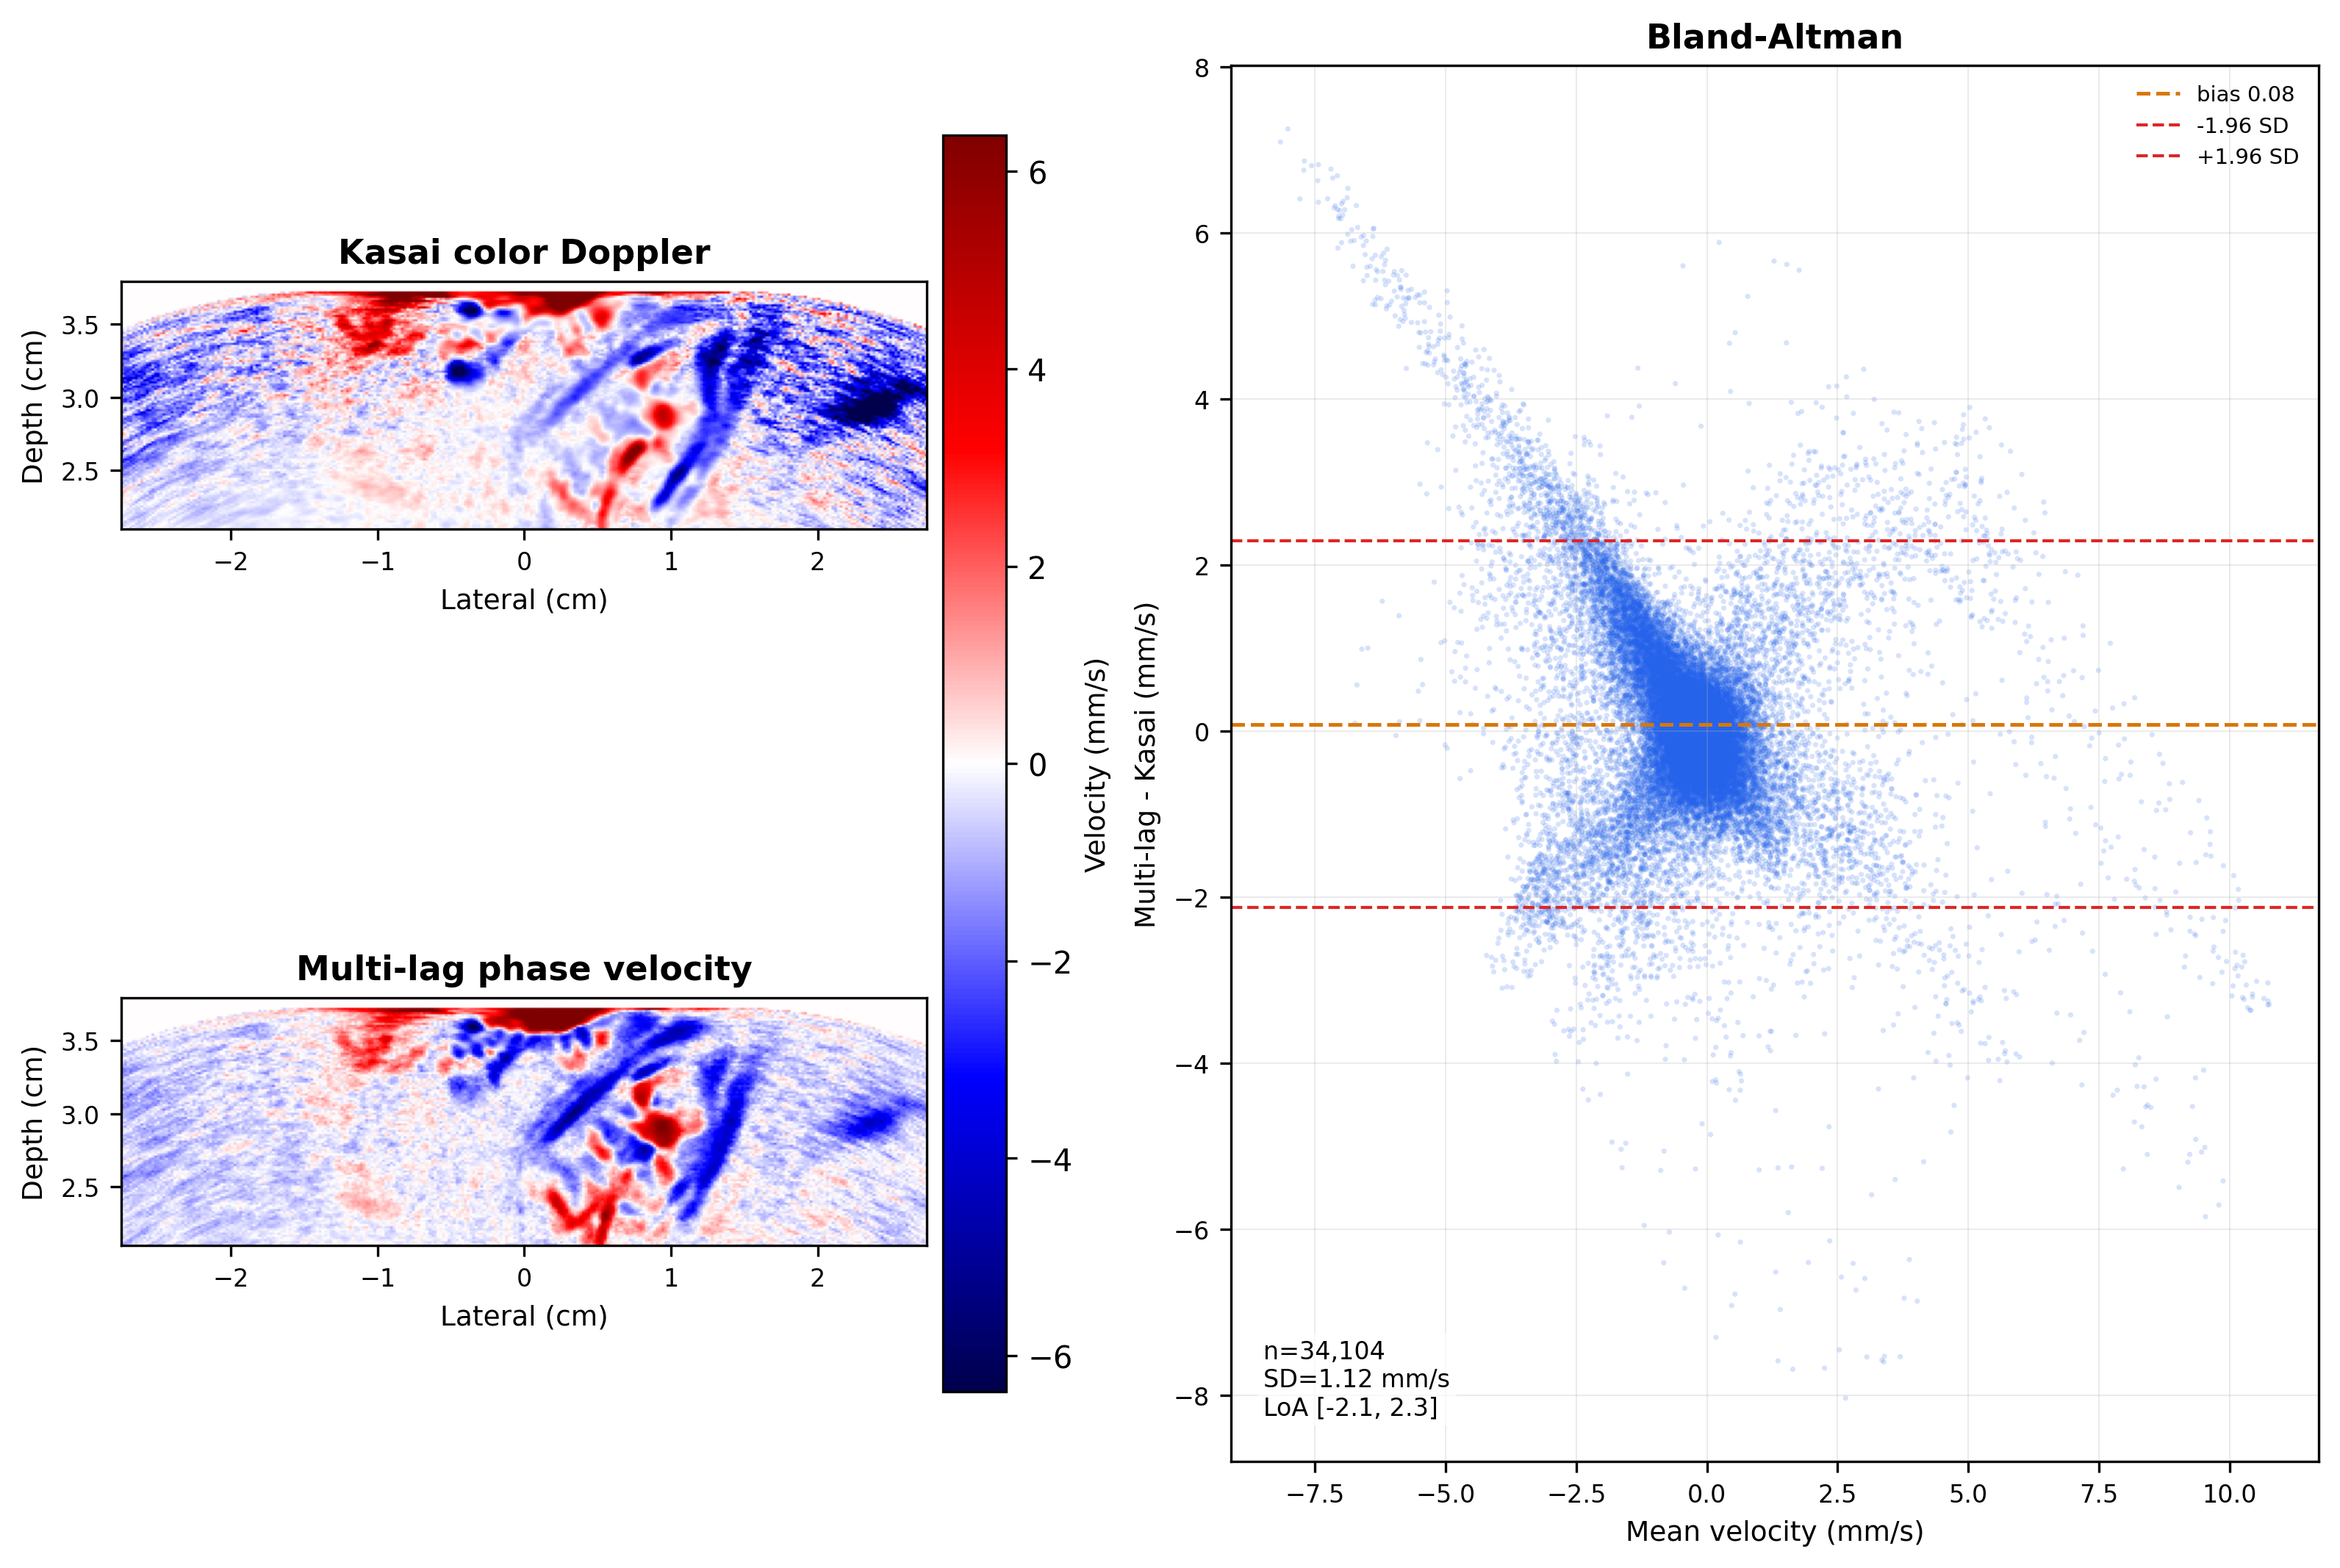
\includegraphics[width=\textwidth]{fig_velocity_vs_color_bland_altman.png}
  \caption{Comparison of conventional lag-1 Kasai color Doppler and
    the multi-lag phase-velocity estimate used by Dower Coppler.
    \textbf{Left}: Kasai velocity, computed from $\angle R_1$.
    \textbf{Center}: multi-lag phase velocity $v_\phi$ from the
    weighted phase-slope fit.  Both velocity maps are shown in
    mm/s with the same symmetric color scale.  \textbf{Right}:
    Bland--Altman plot comparing the two velocity estimates over all
    finite pixels in the displayed plane.}
  \label{fig:velocity_vs_color}
\end{figure*}

\Cref{fig:cnr} quantifies this comparison using contrast-to-noise
ratio (CNR) and generalized CNR (gCNR) across six vessel ROIs
exported from the Doppler CNR viewer.  For each exported signal mask,
we use the largest circular ROI fully contained inside that mask.  The
same vessel-free background rectangle is used for every signal ROI so
that the CNR values differ only because of the selected vessel pixels
and Doppler image.

\begin{figure*}[t]
  \centering
  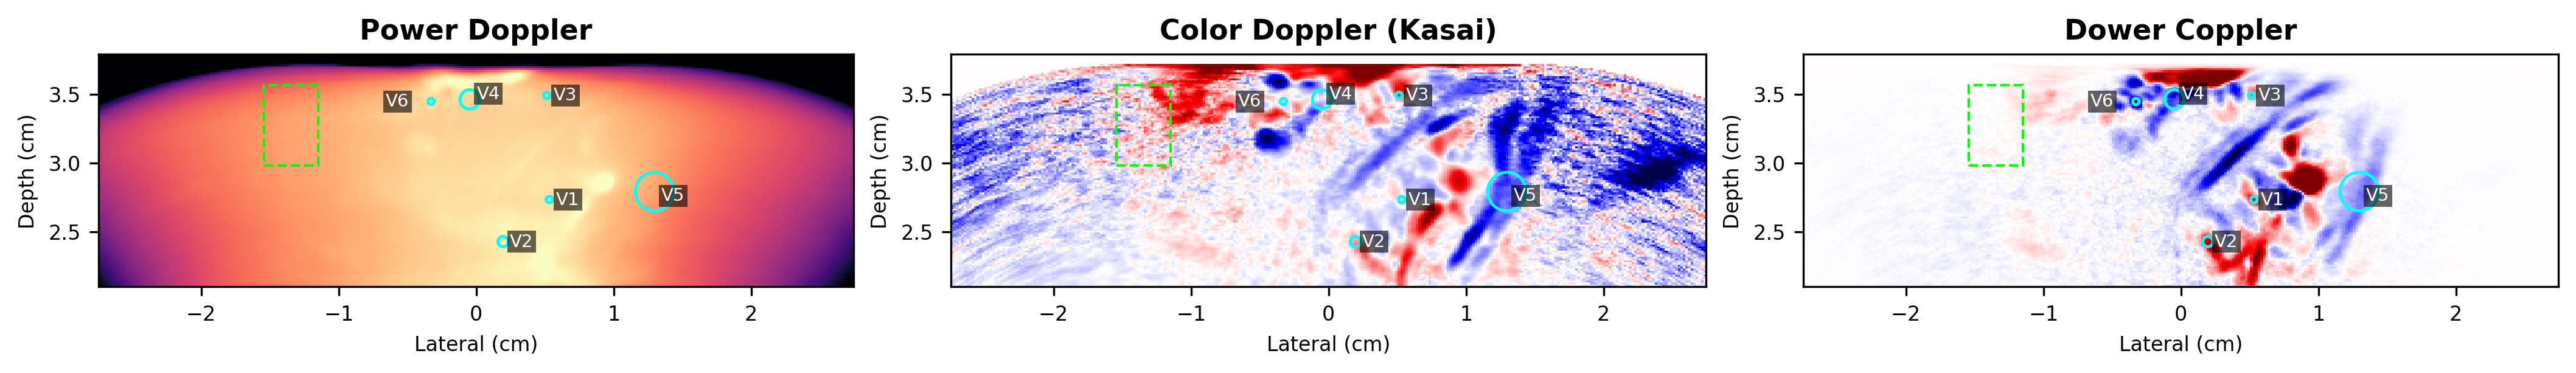
\includegraphics[width=\textwidth]{fig_three_panel_with_rois.png}
  \caption{Regions used for the CNR and gCNR measurements in
    \cref{fig:cnr}.  Cyan circles indicate the largest circular signal
    ROIs fully contained inside the six exported vessel masks.  The
    dashed green rectangle is the shared background ROI used for every
    vessel and every Doppler display.}
  \label{fig:cnr_rois}
\end{figure*}

\begin{figure*}[t]
  \centering
  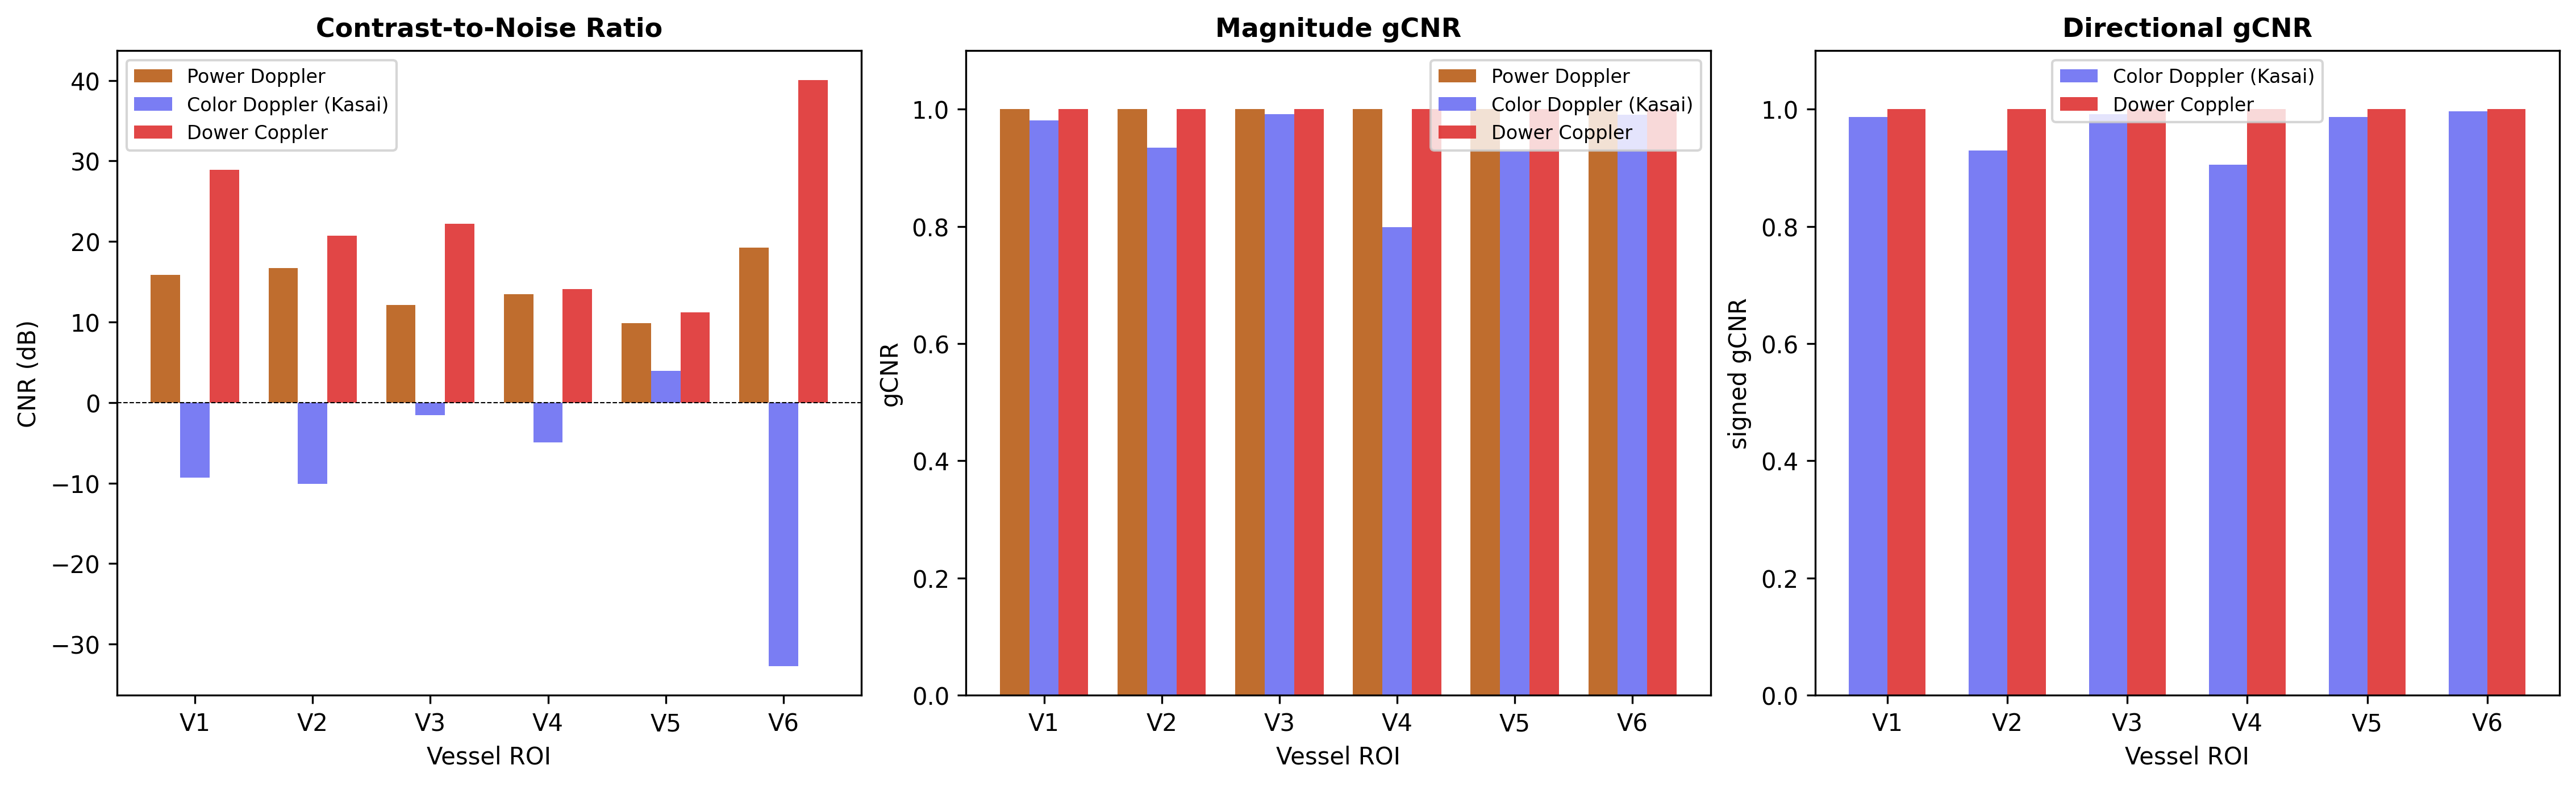
\includegraphics[width=\textwidth]{fig_cnr_comparison.png}
  \caption{\textbf{Left}: CNR in dB across six vessel ROIs.  Dower
    Coppler has median CNR 21.5~dB across the six selections
    (range 11.2--40.1~dB), exceeding both power Doppler and Kasai
    color Doppler in all ROIs.
    \textbf{Middle}: magnitude generalized CNR
    (1~$-$~histogram overlap) using power Doppler, $|$color
    Doppler$|$, and $|$Dower Coppler$|$.
    \textbf{Right}: directional gCNR computed on the signed color
    Doppler and signed Dower Coppler values; power Doppler is omitted
    because it has no direction sign.}
  \label{fig:cnr}
\end{figure*}

Dower Coppler achieves median CNR 21.5~dB across the six largest
inscribed circular vessel selections, with values ranging from
11.2--40.1~dB.  Power Doppler has median CNR 14.7~dB
(range 9.9--19.3~dB), and Kasai color Doppler has median CNR
-7.1~dB (range -32.7--3.9~dB) when the signed Doppler maps are
measured by magnitude, as in the viewer CNR calculation.  The upper
end of the Dower Coppler range is driven by V6, a one-pixel inscribed
circle on a compact high-contrast vessel; we therefore emphasize the
median as the more representative summary statistic.  The gCNR metric
confirms that the selected vessels are well separated from the shared
background region for all three displays when measured by magnitude,
with Dower Coppler and power Doppler at approximately 1.0 across all
selections.  The directional gCNR comparison uses the signed maps
directly and therefore compares only Kasai color Doppler and Dower
Coppler.

As a repeatability check, we split the September 21 acquisitions into
two non-overlapping halves (200--299 and 300--399), recomputed median
Dower Coppler maps from the per-acquisition fine-elevation sidecar,
and compared signs on the closest available elevation plane
($y=-0.44$~mm).  Across the full plane, including low-amplitude
background, the Dower Coppler sign agreed for 68.8\% of 31,810 finite
nonzero pixels.  Restricting the comparison to the highest-magnitude
pixels gave substantially higher agreement: 96.7\% for the top 10\%
of pixels and 98.1\% for the top 5\%.  In the circular vessel ROIs
used for the CNR analysis, the sign was identical between halves for
all 130 vessel-ROI pixels.

\Cref{fig:stability} demonstrates the temporal stability of the Dower
Coppler map by varying the number of acquisitions included in the
median image.

\begin{figure*}[t]
  \centering
  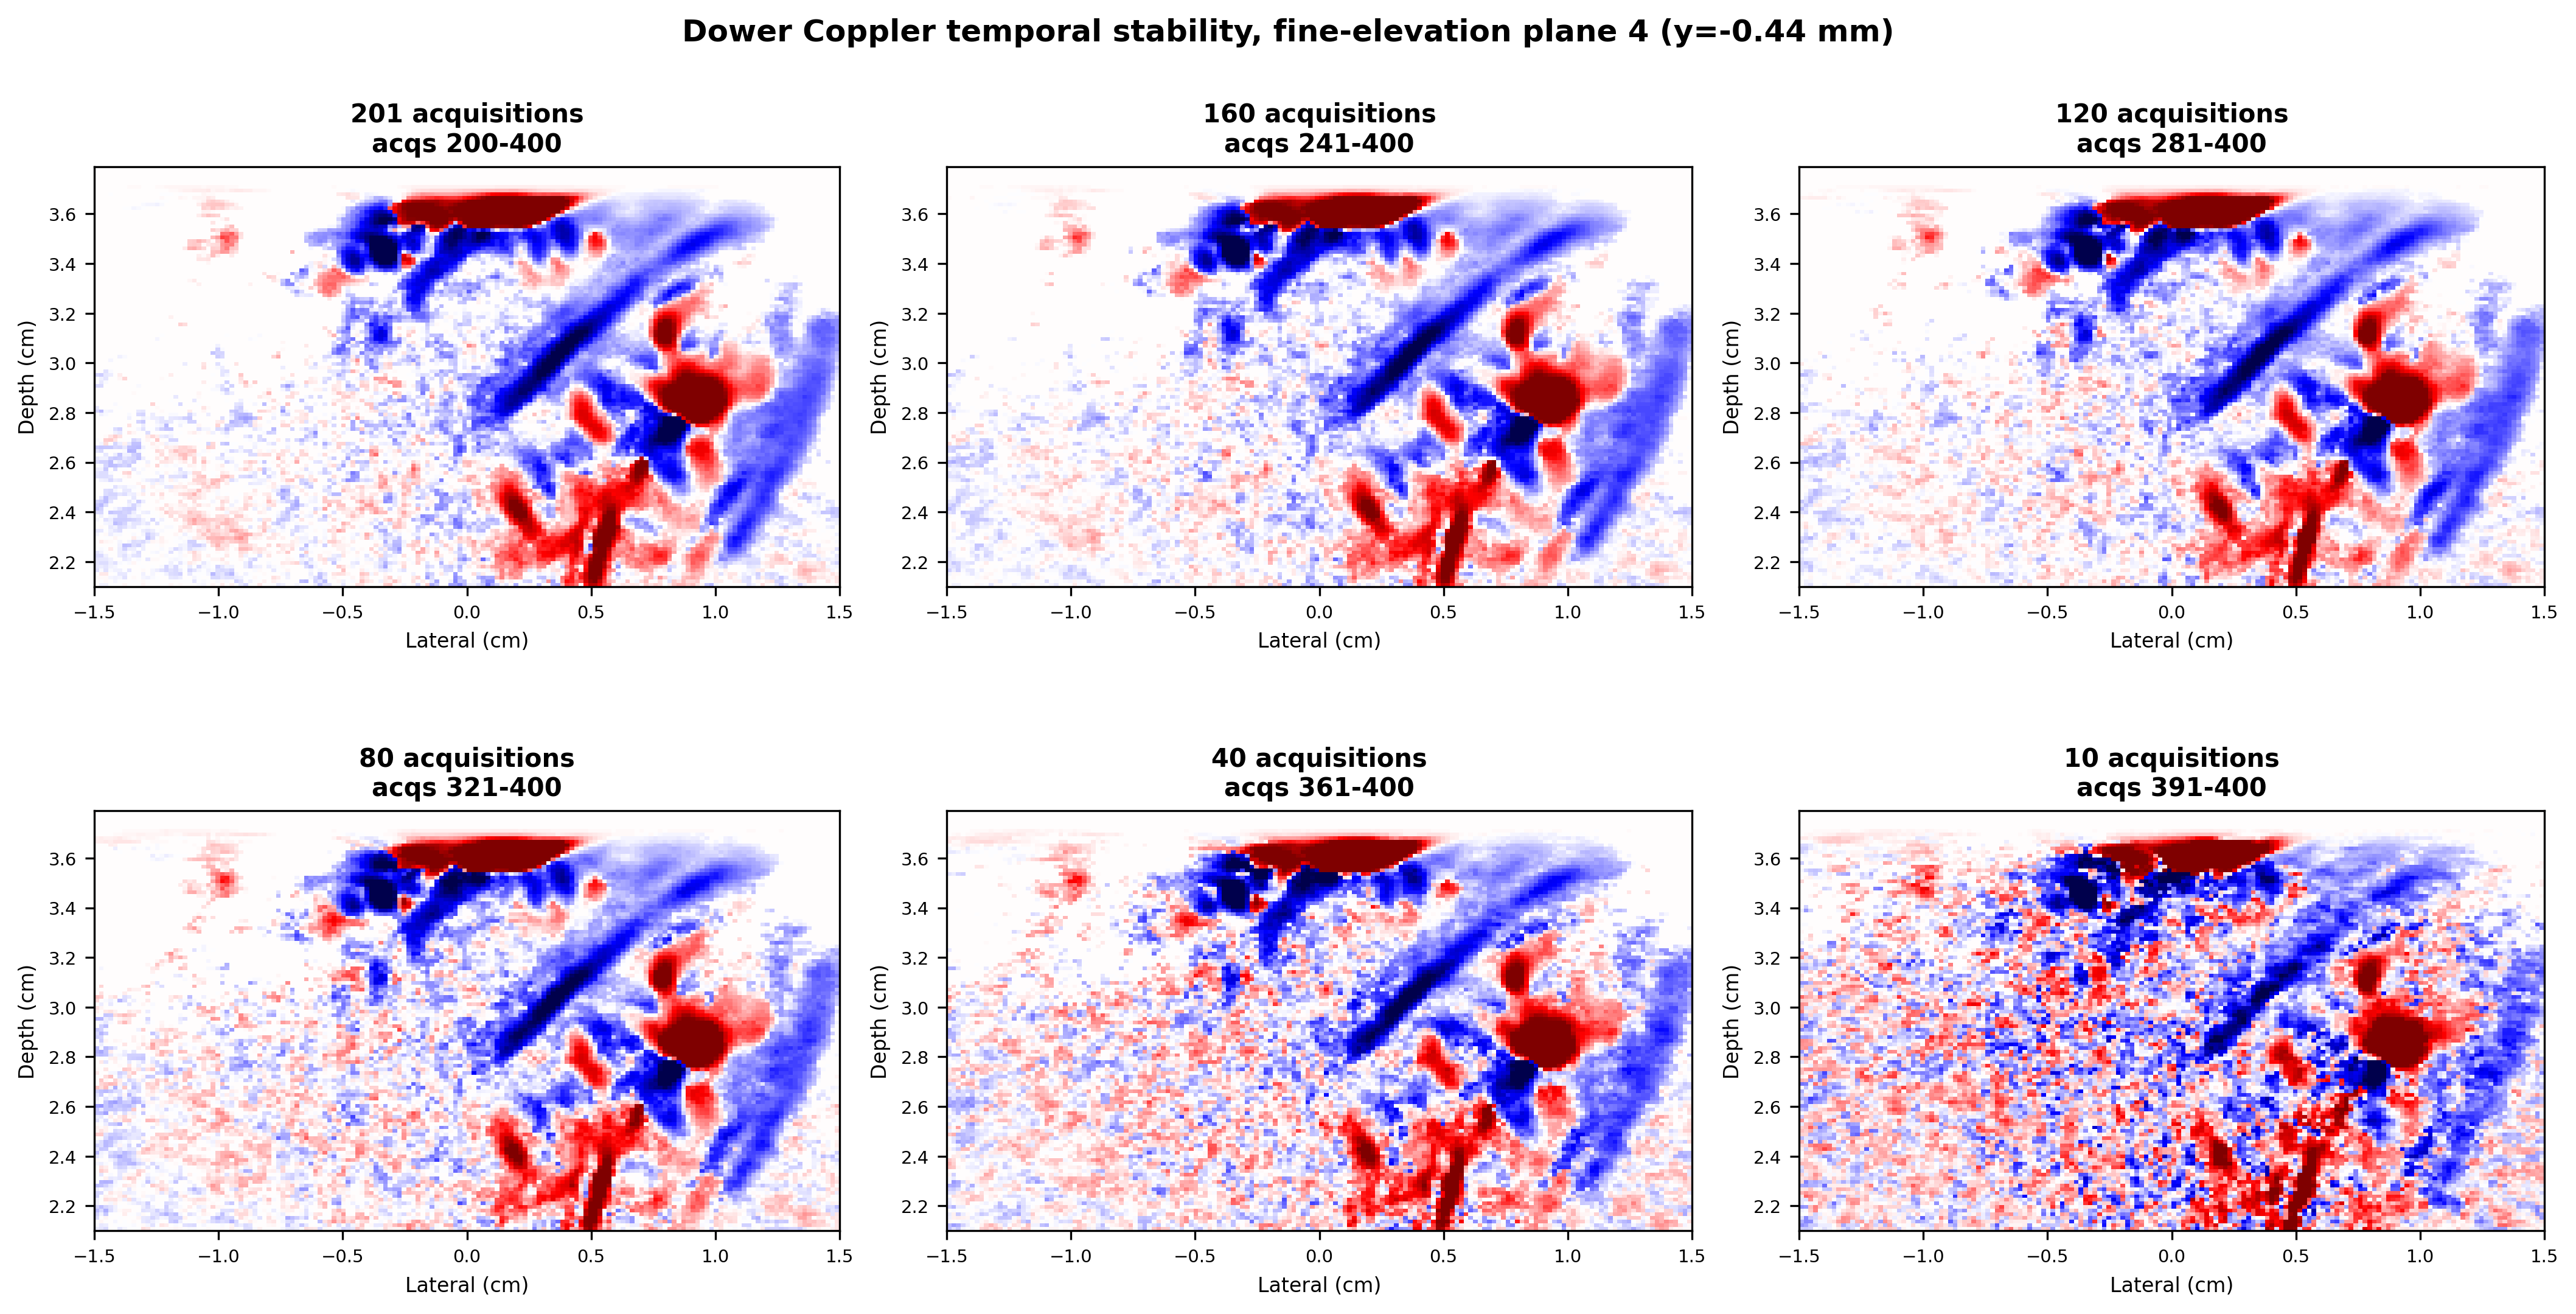
\includegraphics[width=\textwidth]{fig_temporal_stability.png}
  \caption{Dower Coppler maps computed from different numbers of
    acquisitions on the fine-elevation plane at $y=-0.44$~mm.  All
    panels use one shared symmetric color scale.  The vessel pattern
    and flow direction assignment remain stable from 200 acquisitions
    down to 10 acquisitions.  At a single acquisition, the major
    vessels remain identifiable but background noise increases.}
  \label{fig:stability}
\end{figure*}

The vessel pattern and flow direction assignments are stable from 200
acquisitions down to as few as 10 acquisitions.  At a single
acquisition, the major vessels remain identifiable but background
noise increases substantially.

\Cref{fig:all_planes} shows the Dower Coppler map across elevation
planes 2--7 from a finer elevational rebeamforming run spanning
$y=-4$ to $4$~mm, providing a qualitative check that the directional
vascular pattern is not confined to a single selected plane.

\begin{figure*}[t]
  \centering
  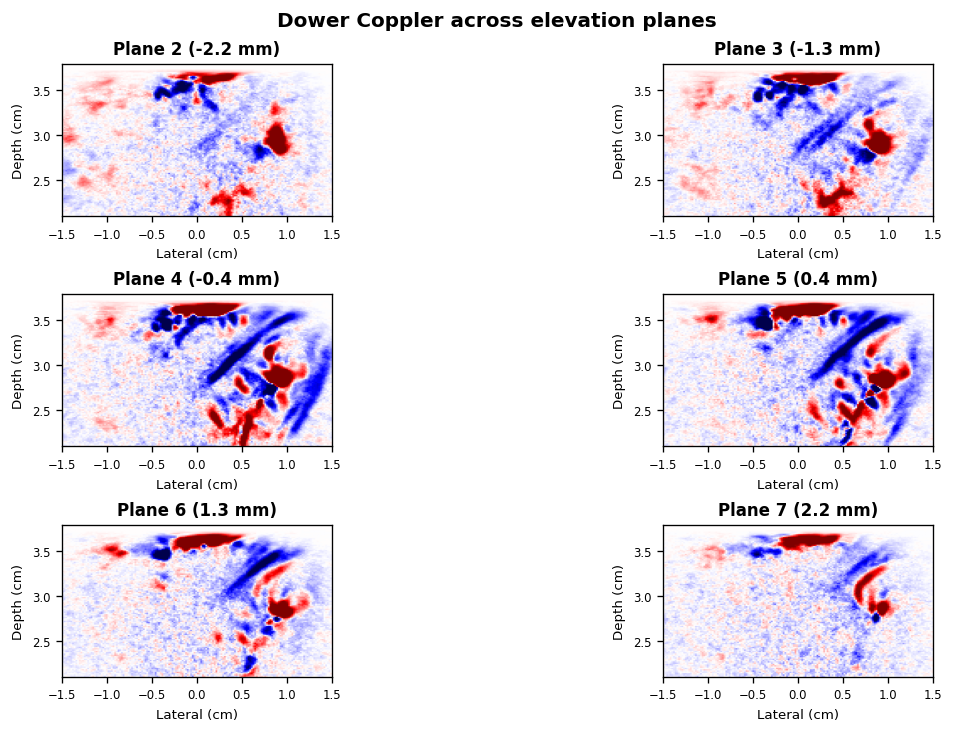
\includegraphics[width=\textwidth,height=0.78\textheight,keepaspectratio]{fig_all_planes.png}
  \caption{Dower Coppler maps across elevation planes 2--7 from the
    finer elevational rebeamforming run spanning $y=-4$ to $4$~mm with
    10 elevation planes.  The panels use acquisitions 200--400 and one
    shared symmetric color scale computed from the 97th percentile of
    absolute Dower Coppler values across the displayed planes.  The directional vascular
    pattern appears across the imaging volume, with similar vessel
    segments visible in adjacent planes.}
  \label{fig:all_planes}
\end{figure*}

\Cref{fig:external_recording} shows the same Dower Coppler processing
on a separate recording, included as a qualitative check that the
displayed vascular contrast is not unique to the September 21 dataset.
The figure-generation script exposes the source NPZ path and elevation
plane as command-line parameters so this example can be replaced
without editing the paper.

\begin{figure}[t]
  \centering
  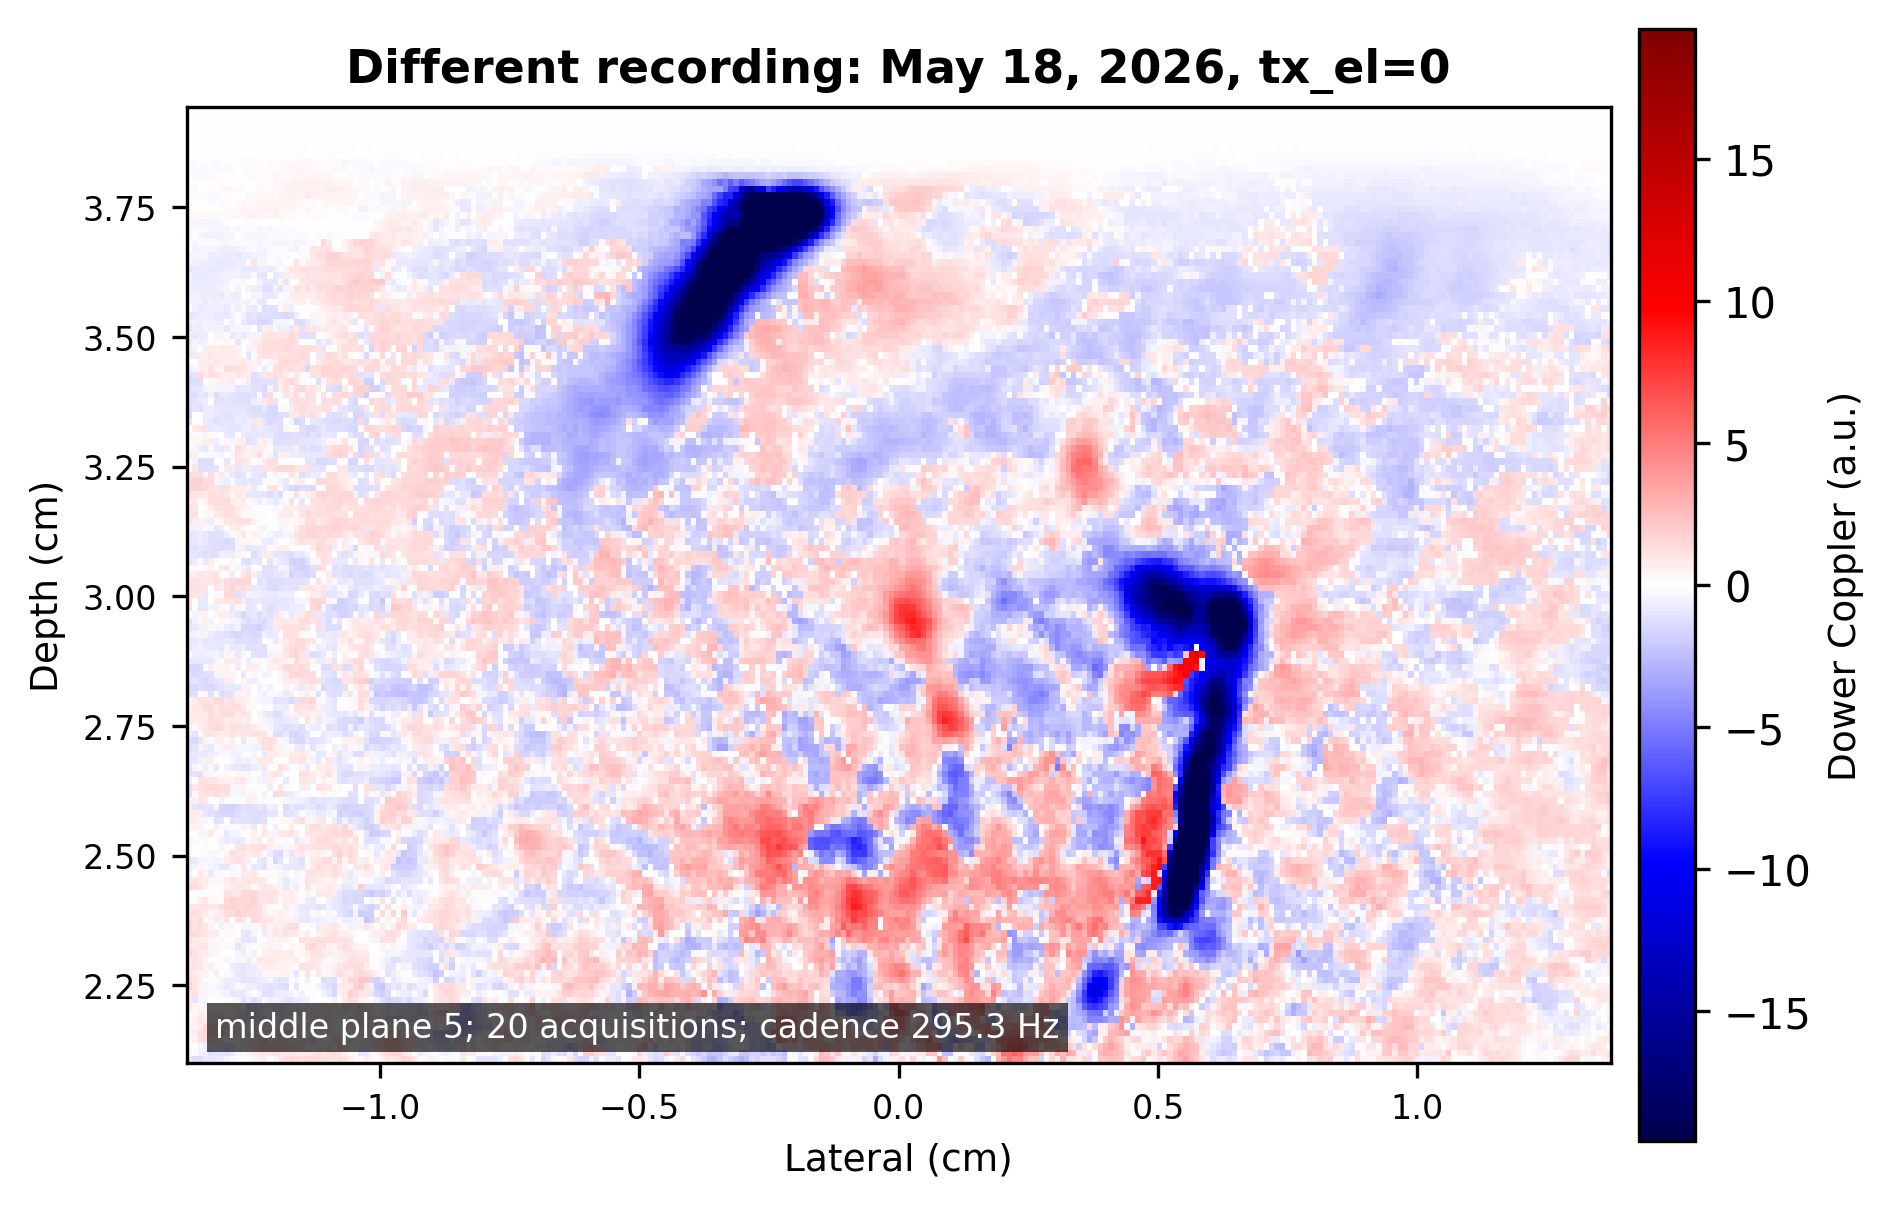
\includegraphics[width=0.82\columnwidth]{fig_external_recording_may18.png}
  \caption{Dower Coppler image from a different recording: May 18,
    2026, BT24480388, transmit element 0.  The displayed image is the
    middle plane from a 10-plane GPU/MACH beamformed H5 ultratrace
    using row\_index=$-1$, $y=-3.5$ to $3.5$~mm, fine lateral/axial
    coarseness 0.5/0.5, 20 acquisitions (0--19), median aggregation,
    PRF 1476.3~Hz, $f_0=2.75$~MHz, $c=1600$~m/s, SVD cutoff 0.08,
    and $K=5$.  The main September 21 dataset uses a separate Head
    ultratrace, acquisitions 200--399 for the CNR/fine-grid analysis,
    elevation planes 2--7 from the $y=-4$ to $4$~mm fine-elevation
    run for the volume montage, pulse PRF 1244.2~Hz
    (compounded-frame cadence 248.8~Hz), and the same $f_0$, $c$, SVD
    cutoff, and $K$.}
  \label{fig:external_recording}
\end{figure}


% ========================================================================
\section{Discussion}
\label{sec:discussion}
% ========================================================================

Dower Coppler is best viewed as a composite Doppler index rather than a
new Doppler estimator from first principles.  Its ingredients---SVD
clutter filtering, complex autocorrelation Doppler, multi-lag phase
estimation, and power-like magnitude weighting---are well established.
The distinct design choice is the scalar product
$v_\phi\,G_R\,R^2$: signed phase velocity multiplied by multi-lag
geometric coherence strength and by phase-linearity quality.  This
hybrid output is signed like color Doppler, amplitude-weighted like
power Doppler, and confidence-gated by the quality of a single
multi-lag phase-slope model.

\paragraph{Relationship to prior work.}
SVD filtering before ultrafast Doppler is standard in fUS and related
microvascular imaging~\cite{demene2015svd}.  Autocorrelation phase
velocity estimation traces directly to Kasai color Doppler
\cite{kasai1985autocorrelation}, and arbitrary temporal/spatial lags
were analyzed in classic color-flow autocorrelation work
\cite{torp1994autocorrelation}.  The Loupas two-dimensional
autocorrelator also uses temporal and depth lags jointly, but for axial
frequency correction rather than multi-lag phase-slope fitting
\cite{loupas1995axial}.  Multi-lag autocorrelation has deep roots in
weather radar, where related estimators fit correlation models across
multiple lags rather than fitting a Doppler phase line
\cite{lei2012multilag,warde2023gmle}.  Frequency estimation from phase
regression is also classical~\cite{tretter1985phaseregression,fitz1994frequency}.
Power Doppler is a close conceptual neighbor because it encodes flow
strength rather than pure velocity~\cite{rubin1994powerdoppler}.  The
TMAS work of Shen and Guo is especially relevant because it directly
uses products of temporal autocorrelation magnitudes to improve
ultrafast power Doppler SNR~\cite{shen2022tmas}; $G_R$ can be
interpreted as a bounded geometric-mean version of this
product-of-lag-magnitudes idea.
Relative to these methods, the contribution here is the specific
coherence-weighted signed index, and in particular the use of a
per-pixel phase-linearity $R^2$ as a confidence gate.  This $R^2$ term
differs from standard spectral-width or variance estimates: it measures
how well the lag phases are explained by one linear slope, penalizing
multi-component flow, turbulence, wrapping errors, and residual clutter.
The claim is therefore not novelty for autocorrelation Doppler, SVD
filtering, or multi-lag correlation processing broadly.

\paragraph{Choice of parameters.}
The maximum lag $K = 5$ was chosen empirically: higher lags provide
more fitting leverage but also more decorrelation, particularly
through the skull.  We used an SVD low cutoff of 0.08, high cutoff of
1.0, mean subtraction before SVD, and omitted the first five filtered
frames from Doppler estimation.  The current implementation uses
weighted least squares rather than Huber reweighting for the final
Dower Coppler image; Huber-derived quality maps remain useful
diagnostics but are not part of the default formula.

\paragraph{Limitations.}
This study uses data from a single volunteer with a single probe.  The
transcranial imaging scenario---with low SNR, strong clutter, and
skull-induced aberrations---is a challenging test case, but validation
on a larger cohort and with flow phantoms providing ground-truth
velocity fields is needed.  Dower Coppler is not itself a quantitative
velocity image: $G_R$ depends on gain, depth attenuation, beamforming
normalization, SVD scaling, and backscatter strength.  Quantitative
velocity analysis should use $v_\phi$ directly, with appropriate
attention to angle dependence and aliasing.  The conversion in
\cref{eq:phase_velocity} estimates the beam-projected axial component;
it does not correct for beam-flow angle.  Multi-lag fitting also does
not remove the fundamental pulse-Doppler phase-wrap ambiguity: the lag
phases still have to be unwrap-able.  Finally, the method assumes a
single dominant flow direction per pixel; bidirectional or turbulent
flow can produce a compromised single-slope estimate, though the $R^2$
term attenuates pixels whose phase sequence is poorly described by a
single velocity.

\paragraph{Extensions.}
The fit quality metric $Q$ is already used as a multiplicative
confidence term, but it can also be displayed as a standalone quality
map.  Robust alternatives, such as Huber-weighted slopes or
circular-sign hybrids, remain useful variants for applications where
isolated lag outliers or sign accuracy dominate the design objective.
Future ablations should explicitly compare power Doppler, Kasai color
Doppler, directional power variants, first-lag magnitude, multi-lag
phase velocity alone, velocity times $G_R$, velocity times $R^2$, and
the full $v_\phi G_R R^2$ index.


% ========================================================================
\section{Conclusion}
\label{sec:conclusion}
% ========================================================================

We have proposed Dower Coppler, a multi-lag coherence-weighted signed
Doppler index for SVD-filtered ultrafast compound ultrasound.  The
method estimates signed beam-projected phase velocity from a multi-lag
autocorrelation phase fit and weights it by lag-correlation strength
and phase-fit quality.  It adds signed directional contrast at minimal
computational cost while attenuating weak or inconsistent pixels.
Simulations show that
multi-lag phase regression reduces frequency estimation error by
2--3$\times$ relative to the single-lag Kasai estimator.
Transcranial \textit{in~vivo} imaging demonstrates that the method
resolves opposing flow directions in adjacent cortical vessels---information
that is lost in conventional power Doppler.

Code, reproducible analysis scripts, and the derived NPZ inputs used
for the manuscript figures are available in the standalone paper
repository:
\href{https://github.com/ennucore/dower-coppler}{github.com/ennucore/dower-coppler}.

\bibliographystyle{unsrtnat}
\bibliography{references}

\end{document}
